\documentclass[12pt,english]{article}
\usepackage[utf8]{inputenc}
\usepackage[a4paper]{geometry}
\geometry{verbose,tmargin=2cm,bmargin=2cm,lmargin=3cm,rmargin=2cm,headheight=12pt,headsep=24pt}
\setcounter{secnumdepth}{3}
\setcounter{tocdepth}{3}
\usepackage{pdfpages}
\usepackage{bm}
\usepackage{array}
\usepackage{float}
\usepackage{graphicx}
\usepackage{tocloft}
\usepackage{hyperref}
\hypersetup{
    colorlinks=true,
    linkcolor=blue,
    filecolor=blue,      
    urlcolor=blue,
}
\usepackage{setspace}
\PassOptionsToPackage{normalem}{ulem}
\usepackage{ulem}
\usepackage{indentfirst}	%Az összes címsor utáni bekezdést beljebb viszi%
\usepackage{amsmath}
\usepackage{tikz}
\usepackage{wrapfig}
\usetikzlibrary{shadings}

\usepackage{pgfplots}


\usepackage{hyperref}
\hypersetup{
    colorlinks,
    citecolor=black,
    filecolor=black,
    linkcolor=black,
    urlcolor=black
}




\makeatletter

%%%%%%%%%%%%%%%%%%%%%%%%%%%%%% LyX specific LaTeX commands.
\newcommand{\noun}[1]{\textsc{#1}}
%% Because html converters don't know tabularnewline
\providecommand{\tabularnewline}{\\}

%%%%%%%%%%%%%%%%%%%%%%%%%%%%%% Textclass specific LaTeX commands.
\newenvironment{lyxcode}
{\par\begin{list}{}{
\setlength{\rightmargin}{\leftmargin}
\setlength{\listparindent}{0pt}% needed for AMS classes
\raggedright
\setlength{\itemsep}{0pt}
\setlength{\parsep}{0pt}
\normalfont\ttfamily}%
 \item[]}
{\end{list}}

%%%%%%%%%%%%%%%%%%%%%%%%%%%%%% User specified LaTeX commands.
%\textwidth 160mm
%\oddsidemargin 0cm
%\topmargin -15mm
\usepackage{bm}
\newcommand{\tg}{\mathop\mathrm{tg}}
\newcommand{\grad}{\mathop\mathrm{grad}}
\newcommand{\BME}{\hrule\vspace{6pt}{\large Budapest University of Technology and Economics
\\
Faculty of Mechanical Engineering \\
Department of Applied Mechanics}}
\newcommand{\szerzo}{}
\newcommand{\konzulensek}{
\parbox[t]{20cm}
{\normalsize
\hspace*{25em} Made by:\\
\hspace*{28em}Bálint CSATÓ\\
\hspace*{25em}Supervisor:\\
\hspace*{28em}Gergely GYEBRÓSZKI \\
}\hfill}

\makeatother

\usepackage{babel}


\begin{document}



\title{\vspace{-2cm}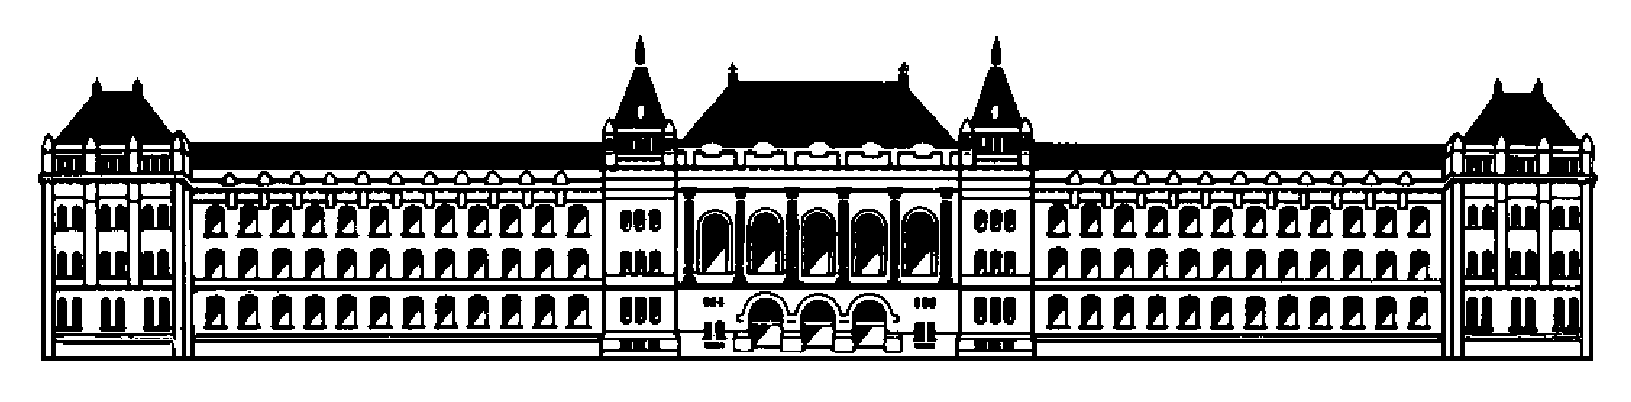
\includegraphics[width=0.4\textwidth,keepaspectratio]{bme_skyline}\\
\BME\vspace{4cm}\\
Control and Parameter Estimation Problems of Autonomous Transport Robots
\\[5mm]
\large{Final Project}}


\author{\sc\szerzo}


\date{\vspace{6cm}\konzulensek\\
\vspace{3cm}Budapest, 2018}

\maketitle
\thispagestyle{empty}



\newpage
\pagenumbering{arabic}
\renewcommand{\contentsname}{Contents}
\renewcommand{\cftsecleader}{\cftdotfill{\cftdotsep}}
\tableofcontents


\newpage
%%%%%%%%%%%%%%%%%%%%%%%%%%%%%%%%%%%%%%%%%%%%%%%%%%%%%%%%%%%%%%%%%%%%%%%%%%%%%%%%%%%%%%%%%%%%%%%%%%%%%%%%%%%%
% 													Preface
%%%%%%%%%%%%%%%%%%%%%%%%%%%%%%%%%%%%%%%%%%%%%%%%%%%%%%%%%%%%%%%%%%%%%%%%%%%%%%%%%%%%%%%%%%%%%%%%%%%%%%%%%%%%
\section*{Preface}
Autonomous vehicle technology offers the possibility of fundamentally
changing transportation. Equipping cars and light vehicles
with this technology will likely reduce crashes, energy consumption,
and pollution and reduce the costs of congestion, as well.

This technology is most easily conceptualized using a five-part
continuum suggested by the National Highway Traffic Safety Administration
(NHTSA), with different benefits of the technology realized
at different levels of automation:
\begin{itemize}
\item \textbf{Level 0:}  The human driver is in complete control of all functions of the car.
\item \textbf{Level 1:}  One function is automated.
\item \textbf{Level 2:}  More than one function is automated at the same time (e.g., steering and acceleration), but the driver must remain constantly attentive.
\item \textbf{Level 3:} The driving functions are sufficiently automated that the driver can safely engage in other activities.
\item \textbf{Level 4:} The car can drive itself without a human driver.
\end{itemize}
\noindent Careful policymaking will be necessary to maximize the social
benefits that this technology will enable, while minimizing the disadvantages[1].


\addcontentsline{toc}{section}{Preface}

\newpage
%%%%%%%%%%%%%%%%%%%%%%%%%%%%%%%%%%%%%%%%%%%%%%%%%%%%%%%%%%%%%%%%%%%%%%%%%%%%%%%%%%%%%%%%%%%%%%%%%%%%%%%%%%%%
% 											Introduction to Autonomous Transport Robots
%%%%%%%%%%%%%%%%%%%%%%%%%%%%%%%%%%%%%%%%%%%%%%%%%%%%%%%%%%%%%%%%%%%%%%%%%%%%%%%%%%%%%%%%%%%%%%%%%%%%%%%%%%%%
\section{Introduction to Autonomous Transport Robots}
\subsection{History of transportation}

Since the early days of the human civilization, one of the most common problem has been the transportation. The first major development was the domestication of animals what made it possible to transport more and heavier loads or humans themselves in order to achieve greater speed and duration. The next substantial invention was the wheel which increased the efficiency of animal transport introducing the concept of vehicles. Until the Industrial Revolution, the water transport facilities proved to be the most effective way. With the development of the combustion engines and automobiles around the end of the 19st century, road transport became competitive again. Today trucks transport cargos over thousands of miles, but light items are still being carried in wheelbarrows or trailers attached to more compact vehicles. 

\begin{figure}[h]
	\centering
	\includegraphics[width=10cm]{evot}
	\label{fig1}
	\caption{Evolution of Transportation}
\end{figure}

\noindent One of the most dominant development tendency in almost every field of the industry is the automation of processes and procedures. Automation means the reduction of human intervention in the operation of machines. The benefit of automation include labor savings, savings in electricity costs, savings in material costs, and improvements to quality, accuracy and precision. The conventional ways of transporting could be appropriate for most of the cases but not in those when repeated passages to specific locations in small distances have to be taken. 
\subsection{Application of autonomous transport robots}
One of the latest trends in technology is to create such driverless robots that can help people in their everyday life, i.e. bringing any kind of products to customers. A company called Starship launched a several self-driving robotic vehicles on the streets of Washington, D.C. that can transport food and other small items to customers ordering via app.
\begin{figure}[h]
	\centering
	\includegraphics[width=5cm]{starship.jpg}
	\label{fig1}
	\caption{Starship Technologies}
\end{figure}
The robotic vehicles move themeselves along sidewalks using camera and tracking technology to avoid any obstacle and its location can be tracked from the distance in order to know the time of arrival. The six-wheeled electric machine sits about a half-meter high having a lockable cargo bay to carry food products up to nine kilograms in weight.\cite{starship}




A company called SMP Robotics made automated guided vehicles that can remove grass clippings and fallen leaves or construct garbage collection in a garden. 
\begin{figure}[h]
	\centering
	\includegraphics[width=5cm]{smp.jpg}
	\label{smp}
	\caption{SMP Robotics}
\end{figure}

\noindent These small-sized mobile robots have a trailer attached to the back. They are powered by electrical engines, thus noise and smell emission is minimized which allow for operation around people. The built-in accumulators stores the needed energy and can last for several days of cyclical operation. Two ways of route following method is available. The first option is to choose a root in advance with the help of the attached PC tablet. The second way is to set the robot in its 'follow me' algorithm whereby it is going to follow the operator and learn the path. The collected goods on the trailer can be unloaded automatically using a mechanism without any human intervention. The trailer can be fitted with a water tank which can be used for watering of grass and other plants, furthermore automatic water refill algorithm is implemented. This kind of automatic self-moving watering system suits really well such occasions when a fixed irrigation systems are not worth being built due to climate characteristics.\cite{smp}

A firm named NEOBOTIX made autonomous transport system for daily use in industrial applications. The robots are equipped with laser scanners that permanently detect landmarks and obstacles what allows the robot to react dynamically to unexpected changes of their surrounding, i.e. to safely operate between human and other moving objects. This flexibility makes them suited for dynamic transportation tasks with frequent changes. For instance, they can complement roller or belt conveyors and take parts to machines or workplaces that are not connected to the conveyor system. \cite{neo}

\begin{figure}[h]
	\centering
	\minipage{0.40\textwidth}
	\centering
	\includegraphics[height=5cm]{neo1.jpg}
	\caption{{\small MT-400}}
	\endminipage\hfill
	\minipage{0.40\textwidth}
	\centering
	\includegraphics[height=5cm]{neo2.jpg}
	\caption{{\small MT-500}}
	\label{conv2}
	\endminipage\hfill
\end{figure} 

\noindent Possible applications are taking parts to and from workplaces, transporting in direct interaction with humans or dynamic picking of parts for later assembly

BMW logistics also uses autonomous transport robots similarly in industrial environment. The well-known car manufacturer has been working hard to reduce emissions in all steps of the manufacturing process of a car, not only in the final product. This application shows really well that the autonomous developments in the automotive industry is not just about the autonomous driving on the roads but the manufacturing processes as well. Smart Transport Robots (STR) transport components through logistics at the Wackersdorf plant. They measures the distance to wireless transmitters which are located at in the logistics hall to calculate its exact position and route. Using sensors to identify and react to critical situations, it is able to share the route with humans and other vehicles. \cite{bmw}

\begin{figure}[h]
	\centering
	\includegraphics[width=7cm]{bmw.jpg}
	\label{bmw}
	\caption{BMW: Smart Transport Robots}
\end{figure}

Another interesting field of application of transportation robots is the military. By putting humans to this work they are often exposed to a risk that could be avoided.The Autonomous Platform Demonstrator is a military transportation robot developed by the U.S. It has a hybrid-electric drive train with six in-hub electric motors powered by li-ion batteries charged using an on-board diesel generator. From control point of view it can be controlled in real-time by a soldier or it can operate autonomously. Autonomously it can operate at speeds up to 50 mph. It can travel along a GPS way point route and avoid obstacles in its way. \cite{apd}

\begin{figure}[h]
	\centering
	\includegraphics[width=7cm]{apd.jpg}
	\label{bmw}
	\caption{Military transportation robot: APD}
\end{figure}


\newpage	
\section{Mobile Robots}
hfdhdhf












%%%%%%%%%%%%%%%%%%%%%%%%%%%%%%%%%%%%%%%%%%%%%%%%%%%%%%%%%%%%%%%%%%%%%%%%%%%%%%%%%%%%%%%%%%%%%%%%%%%%%%%%%%%%
% 											Bibliography
%%%%%%%%%%%%%%%%%%%%%%%%%%%%%%%%%%%%%%%%%%%%%%%%%%%%%%%%%%%%%%%%%%%%%%%%%%%%%%%%%%%%%%%%%%%%%%%%%%%%%%%%%%%%

\newpage
\begin{thebibliography}{1}

\addcontentsline{toc}{section}{References}

\bibitem {c} 
James M. Anderson, Nidhi Kalra, Karlyn D. Stanley, Paul Sorensen, Constantine Samaras, Oluwatobi A. Oluwatola: \emph{Autonomous Vehicle Technology}


\bibitem {smp} 
SMP Robotics: https://smprobotics.com/ \href{https://smprobotics.com/application_autonomus_mobile_robots/transport-robots/}{[link]}

\bibitem {starship} 
Starship Technologies: https://www.starship.xyz/ \href{https://www.starship.xyz/}{[link]}

\bibitem {neo} 
NEOBOTIX: https://http://www.neobotix-robots.com/ \href{http://www.neobotix-robots.com/}{[link]}

\bibitem {bmw} 
BMW STR: http://www.bmwblog.com/ \href{http://www.bmwblog.com/2016/11/18/bmw-logistics-now-use-autonomous-transport-robots/}{[link]}

\bibitem {apd} 
Allonrobots: http://www.allonrobots.com/military-transportation-robots.html \href{http://www.allonrobots.com/military-transportation-robots.html}{[link]}



\bibitem{whatisarduino} Alan G. Smith: \emph{Introduction to Arduino, 2011}


\bibitem{communication_arduino} Brian W. Evans: \emph{Arduino Programming Notebook, 2007}


\bibitem{i2c_communication_arduino} Alex Lange: \emph{I2C Communication with Arduino, 2015}

\bibitem{i2C_communication_arduino_2} http://howtomechatronics.com \href{http://howtomechatronics.com/}{[link]}

	\bibitem{orientation_arduino} Kevin Townsend: \emph{Adafruit BNO055 Absolute Orientation Sensor, 2017}

	\bibitem{optical flow} https://github.com/Lauszus/ADNS3080 \href{https://github.com/Lauszus/ADNS3080}{[link]}
	
\end{thebibliography}

\end{document}
